\let\negmedspace\undefined
\let\negthickspace\undefined
\documentclass[journal]{IEEEtran}
\usepackage[a4paper, margin=10mm, onecolumn]{geometry}
\usepackage{lmodern} % Ensure lmodern is loaded for pdflatex
\usepackage{tfrupee} % Include tfrupee package

\setlength{\headheight}{1cm} % Set the height of the header box
\setlength{\headsep}{0mm}  % Set the distance between the header box and the top of the text

\usepackage{gvv-book}
\usepackage{gvv}
\usepackage{cite}
\usepackage{amsmath,amssymb,amsfonts,amsthm}
\usepackage{algorithmic}
\usepackage{graphicx}
\usepackage{float}
\usepackage{textcomp}
\usepackage{xcolor}
\usepackage{txfonts}
\usepackage{listings}
\usepackage{enumitem}
\usepackage{mathtools}
\usepackage{gensymb}
\usepackage{comment}
\usepackage[breaklinks=true]{hyperref}
\usepackage{tkz-euclide} 
\usepackage{listings}
% \usepackage{gvv}                                        
\def\inputGnumericTable{}                                 
\usepackage[latin1]{inputenc}                                
\usepackage{color}                                            
\usepackage{array}                                            
\usepackage{longtable}                                       
\usepackage{calc}                                             
\usepackage{multirow}                                         
\usepackage{hhline}                                           
\usepackage{ifthen}                                           
\usepackage{lscape}
\usepackage{tikz}
\usetikzlibrary{patterns}

\begin{document}

\bibliographystyle{IEEEtran}
\vspace{3cm}

\title{6.3.4}
\author{EE25BTECH11064 - Yojit Manral}

\maketitle
% \maketitle
% \newpage
% \bigskip
{\let\newpage\relax\maketitle}
\renewcommand{\thefigure}{\theenumi}
\renewcommand{\thetable}{\theenumi}
\setlength{\intextsep}{10pt} % Space between text and float

\textbf{Question:}

Find the shortest distance between the lines
\begin{align}
    \vec{r}&=(\vec{i}+2\vec{j}+\vec{k})+\kappa_1(\vec{i}-\vec{j}+\vec{k}) \\
    \vec{r}&=(2\vec{i}-\vec{j}-\vec{k})+\kappa_2(2\vec{i}+\vec{j}+2\vec{k})
\end{align}

\textbf{Solution:}

$\longrightarrow$ The lines can be represented in vector form as
\begin{align}
    L_1 \equiv \vec{x} = \vec{A} + \kappa_1\vec{m_1} = \myvec{1\\2\\1} + \kappa_1\myvec{1\\-1\\1} \\
    L_2 \equiv \vec{x} = \vec{B} + \kappa_2\vec{m_2} = \myvec{2\\-1\\-1} + \kappa_2\myvec{2\\1\\2} 
\end{align}
$\rightarrow$ To check whether the given lines are skewed
\begin{align}
    \vec{M} = \myvec{\vec{m_1}&\vec{m_2}} = \myvec{1&2\\-1&1\\1&2}, &\vec{B}-\vec{A} = \myvec{1\\-3\\-2} \\
    \myvec{1&2&1\\-1&1&-3\\1&2&-2}\xrightarrow[R_3 \leftrightarrow R_3 - R_1]{R_2 \leftrightarrow R_2 + R_1}&\myvec{1&2&1\\0&3&-2\\0&0&-3} \\
    rank\myvec{\vec{M}&\vec{B}-\vec{A}} = 3 \implies& \text{ The given lines are skew}
\end{align}

$\longrightarrow$ Let $x_1(\mu_1)$ and $x_2(\mu_2)$ be the points closest to each other from the lines $L_1$ and $L_2$, respectively
\begin{align}
     \vec{x_1} = \vec{A} + \mu_1\vec{m_1} &&
     \vec{x_2} = \vec{B} + \mu_2\vec{m_2}
\end{align}
$\rightarrow$ Now, we have
\begin{align}
    (\vec{x_1}-\vec{x_2})^T\vec{m_1} = (\vec{x_1}-\vec{x_2})^T\vec{m_2} = 0 \\
    (\vec{x_1}-\vec{x_2})^T \myvec{\vec{m_1}&\vec{m_2}} = 0\\
    \vec{M}^T (\vec{x_1}-\vec{x_2}) = 0
\end{align}
$\rightarrow$ Using the \textit{least squares method}
\begin{align}
    \vec{x_1}-\vec{x_2} &= \vec{A}-\vec{B}+\myvec{\vec{m_1}&\vec{m_2}}\myvec{\mu_1\\-\mu_2} \\
    0 &= \vec{M}^T(\vec{A}-\vec{B})+\vec{M}^T\vec{M}\myvec{\mu_1\\-\mu_2} \\
    \vec{M}^T\vec{M}\vec{\mu} &= \vec{M}^T(\vec{B}-\vec{A}),\hspace{0.2cm} \vec{\mu} = \myvec{\mu_1\\-\mu_2}
\end{align}

$\longrightarrow$ To perform \textit{singular value decomposition}, we do the following eigen-decompositions
\begin{align}
    \vec{M}^T\vec{M} = \myvec{3&3\\3&9} = \vec{V}\vec{D_2}\vec{V}^T \\
    \vec{M}\vec{M}^T = \myvec{5&1&5\\1&2&1\\5&1&5} = \vec{U}\vec{D_1}\vec{U}^T 
\end{align}
$\rightarrow$ For $\vec{M}^T\vec{M}$, the characteristic polynomial is
\begin{align}
    char(\vec{M}^T\vec{M}) = \left|\begin{array}{cc}3-\lambda&3\\3&9-\lambda\end{array}\right| = \lambda^2 - 12\lambda + 18 
    \implies \lambda_1 = 6 + 3\sqrt{2}, \lambda_2 = 6 - 3\sqrt{2}
\end{align}
$\rightarrow$ For $\lambda_1$, the augmented matrix formed using the eigenvalue-eigenvector equation gives
\begin{align}
    \myvec{-3-3\sqrt{2}&3\\3&3-3\sqrt{2}}\xleftrightarrow{\text{which simplifies to}}\myvec{1&1-\sqrt{2}\\0&0} \\
    \implies \vec{v_1} = k\myvec{-1+\sqrt{2}\\1} = \frac{1}{\sqrt{4-2\sqrt{2}}}\myvec{-1+\sqrt{2}\\1}
\end{align}
$\rightarrow$ For $\lambda_2$, the augmented matrix formed using the eigenvalue-eigenvector equation gives
\begin{align}
    \myvec{-3+3\sqrt{2}&3\\3&3+3\sqrt{2}}\xleftrightarrow{\text{which simplifies to}}\myvec{1&1+\sqrt{2}\\0&0} \\
    \implies \vec{v_2} = k\myvec{-1-\sqrt{2}\\1} = \frac{1}{\sqrt{4+2\sqrt{2}}}\myvec{-1-\sqrt{2}\\1}
\end{align}
$\rightarrow$ Using (15), we get
\begin{align}
    \vec{V} = \myvec{\vec{v_1}&\vec{v_2}} &= \myvec{\frac{-1+\sqrt{2}}{\sqrt{4-2\sqrt{2}}}&\frac{-1-\sqrt{2}}{\sqrt{4+2\sqrt{2}}} \\ \frac{1}{\sqrt{4-2\sqrt{2}}}&\frac{1}{\sqrt{4+2\sqrt{2}}}} \\
    \vec{D_2} &= \myvec{6+3\sqrt{2}&0\\0&6-3\sqrt{2}}
\end{align}
$\rightarrow$ For $\vec{M}\vec{M}^T$, the characteristic polynomial is
\begin{align}
    char(\vec{M}\vec{M}^T) = \left|\begin{array}{ccc}5-\lambda&1&5\\1&2-\lambda&1\\5&1&5-\lambda\end{array}\right| = \lambda(\lambda^2 - 12\lambda + 18)
    \implies \lambda_1 = 6 + 3\sqrt{2}, \lambda_2 = 6 - 3\sqrt{2}, \lambda_3 = 0
\end{align}
$\rightarrow$ For $\lambda_1$, the augmented matrix formed using the eigenvalue-eigenvector equation gives
\begin{align}
    \myvec{-1-3\sqrt{2}&1&5\\1&-4-3\sqrt{2}&1\\5&1&-1-3\sqrt{2}}\xleftrightarrow{\text{which simplifies to}}\myvec{1&0&-1\\0&1&4-3\sqrt{2}\\0&0&0} \\
    \implies \vec{u_1} = k\myvec{1\\-4+3\sqrt{2}\\1} = \frac{1}{\sqrt{36-24\sqrt{2}}}\myvec{1\\-4+3\sqrt{2}\\1} = \frac{1}{\sqrt{12}}\myvec{1+\sqrt{2}\\2-\sqrt{2}\\1+\sqrt{2}}
\end{align}
$\rightarrow$ For $\lambda_2$, the augmented matrix formed using the eigenvalue-eigenvector equation gives
\begin{align}
    \myvec{-1+3\sqrt{2}&1&5\\1&-4+3\sqrt{2}&1\\5&1&-1+3\sqrt{2}}\xleftrightarrow{\text{which simplifies to}}\myvec{1&0&-1\\0&1&4+3\sqrt{2}\\0&0&0} \\
    \implies \vec{u_2} = k\myvec{1\\-4-3\sqrt{2}\\1} = \frac{-1}{\sqrt{36+24\sqrt{2}}}\myvec{1\\-4-3\sqrt{2}\\1} = \frac{1}{\sqrt{12}}\myvec{1-\sqrt{2}\\2+\sqrt{2}\\1-\sqrt{2}}
\end{align}
$\rightarrow$ For $\lambda_3$, the augmented matrix formed using the eigenvalue-eigenvector equation gives
\begin{align}
    \myvec{5&1&5\\1&2&1\\5&1&5}\xleftrightarrow{\text{which simplifies to}}\myvec{1&0&1\\0&1&0\\0&0&0} \\
    \implies \vec{u_3} = k\myvec{-1\\0\\1} = \frac{1}{\sqrt{2}}\myvec{-1\\0\\1}
\end{align}
$\rightarrow$ Using (16), we get the following
\begin{align}
    \vec{U} = \myvec{\vec{u_1}&\vec{u_2}&\vec{u_3}} &= \myvec{\frac{1+\sqrt{2}}{\sqrt{12}}& \frac{1-\sqrt{2}}{\sqrt{12}}&-\frac{1}{\sqrt{2}}\\\frac{2-\sqrt{2}}{\sqrt{12}}&\frac{2+\sqrt{2}}{\sqrt{12}}&0\\\frac{1+\sqrt{2}}{\sqrt{12}}&\frac{1-\sqrt{2}}{\sqrt{12}}&\frac{1}{\sqrt{2}}} \\
    \implies \vec{U_R} &= \myvec{\frac{1+\sqrt{2}}{\sqrt{12}}&\frac{1-\sqrt{2}}{\sqrt{12}}\\\frac{2-\sqrt{2}}{\sqrt{12}}&\frac{2+\sqrt{2}}{\sqrt{12}}\\\frac{1+\sqrt{2}}{\sqrt{12}}&\frac{1-\sqrt{2}}{\sqrt{12}}} \\
    \vec{D_1} &= \myvec{6+3\sqrt{2}&0&0\\0&6-3\sqrt{2}&0\\0&0&0}
\end{align}

$\longrightarrow$ Then, for using \textit{singular value decomposition}, we define
\begin{align}
\vec{\Sigma} \triangleq \myvec{\sqrt{6+3\sqrt{2}}&0\\0&\sqrt{6-3\sqrt{2}}\\0&0} \implies
\vec{\Sigma_R} \triangleq \myvec{\sqrt{6+3\sqrt{2}}&0\\0&\sqrt{6-3\sqrt{2}}}
\end{align}
$\rightarrow$ Using \textit{singular value decomposition} and substituting in (14)
\begin{align}
    \vec{M} &= \vec{U_R}\vec{\Sigma_R}\vec{V}^T \\
    \vec{V}\vec{\Sigma_R}^T\vec{U_R}^T\vec{U_R}\vec{\Sigma_R}\vec{V}^T\vec{\mu} &= \vec{V}\vec{\Sigma_R}^T\vec{U_R}^T(\vec{B}-\vec{A}) \\
    \vec{V}\vec{\Sigma_R}^2\vec{V}^T\vec{\mu} &= \vec{V}\vec{\Sigma_R}\vec{U_R}^T(\vec{B}-\vec{A}) \\
    \vec{\mu} &= (\vec{V}\vec{\Sigma_R}^2\vec{V}^T)^{-1}\vec{V}\vec{\Sigma_R}\vec{U_R}^T(\vec{B}-\vec{A}) \\
    \vec{\mu} &= \vec{V}\vec{\Sigma_R}^{-2}\vec{V}^T\vec{V}\vec{\Sigma_R}\vec{U_R}^T(\vec{B}-\vec{A}) \\
    \vec{\mu} &= \vec{V}\vec{\Sigma_R}^{-1}\vec{U_R}^T(\vec{B}-\vec{A})
\end{align}
$\rightarrow$ Putting the required values in (40)
\begin{align}
    \vec{\mu} = \myvec{\frac{-1+\sqrt{2}}{\sqrt{4-2\sqrt{2}}}&\frac{-1-\sqrt{2}}{\sqrt{4+2\sqrt{2}}} \\ \frac{1}{\sqrt{4-2\sqrt{2}}}&\frac{1}{\sqrt{4+2\sqrt{2}}}} \myvec{\frac{1}{\sqrt{6+3\sqrt{2}}}&0\\0&\frac{1}{\sqrt{6-3\sqrt{2}}}} \myvec{\frac{1+\sqrt{2}}{\sqrt{12}}&\frac{2-\sqrt{2}}{\sqrt{12}}&\frac{1+\sqrt{2}}{\sqrt{12}}\\\frac{1-\sqrt{2}}{\sqrt{12}}&\frac{2+\sqrt{2}}{\sqrt{12}}&\frac{1-\sqrt{2}}{\sqrt{12}}} \myvec{1\\-3\\-2} \\
    \myvec{\mu_1\\-\mu_2} = \myvec{\frac{-1+\sqrt{2}}{\sqrt{12}}&\frac{-1-\sqrt{2}}{\sqrt{12}}\\\frac{1}{\sqrt{12}}&\frac{1}{\sqrt{12}}} \myvec{\frac{-7+2\sqrt{2}}{\sqrt{12}}\\\frac{-7-2\sqrt{2}}{\sqrt{12}}} = \myvec{11/6\\-7/6} \implies \myvec{\mu_1\\\mu_2} = \myvec{11/6\\7/6}
\end{align}

$\longrightarrow$ This gives us the vector coordinates of $x_1$ and $x_2$, as
\begin{align}
\vec{x_1} = \myvec{1\\2\\1} + \brak{\frac{11}{6}}\myvec{1\\-1\\1} = \myvec{17/6\\1/6\\17/6} &&
\vec{x_2} = \myvec{2\\-1\\-1} + \brak{\frac{7}{6}}\myvec{2\\1\\2} = \myvec{26/6\\1/6\\8/6}
\end{align}
$\rightarrow$ And the least distance as
\begin{align}
    \norm{\vec{x_1}-\vec{x_2}}=\norm{\myvec{-3/2\\0\\3/2}}=\frac{3\sqrt{2}}{2}
\end{align}
\begin{figure}[h!]
   \centering
   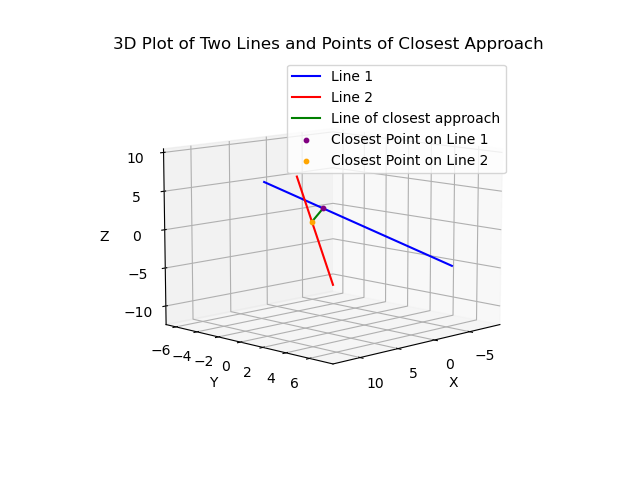
\includegraphics[width=\linewidth]{figs/01.png}
   \caption{Plot of given lines and shortest distance between them}
   \label{Plot_1}
\end{figure}
\end{document}
